\subsection{Part 1}
\subsubsection{Task 1}
Initialize the repository.
\begin{figure}[H]
    \centering
    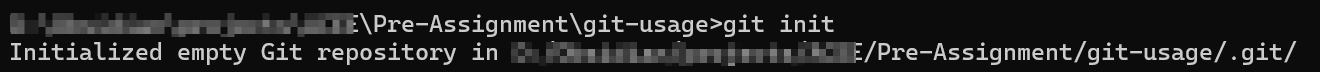
\includegraphics[width = \textwidth]{./figures/init.png}
    \caption{use `git init' to initialize the repository}
\end{figure}

Add the file `test1.txt' `test2.txt' as the new file.
\begin{figure}[H]
\centering
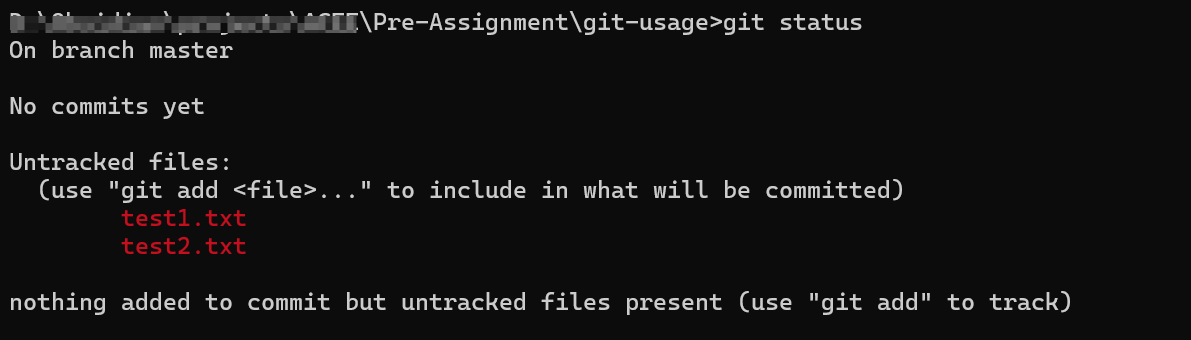
\includegraphics[width = \textwidth]{./figures/status.png}
\caption{use `git status' to check out status of all files}
\end{figure}

\textbf{Question}: What changes after tracking your file? Write down your comprehension of status of eachfile. (Untracked,Modified,Staged,Committed)

\textbf{Answer}: After tracking my file, the status is transformed from `Untracked' to `Staged'.
\begin{itemize}
    \item Untracked:

    The file is new and it's not under the control of git. Git will not track its changes. If you want to stage it, you can use `git add <file name>' to turn it into staged.

    \item Modified:

    The file is tracked, but modified. It differs from the latest version of the one in repository. You can use `git add <file name>' to stage it.

    \item Staged:

    The file is ready to commit and is storaged in the `Staging Area'.

    \item Committed:

    The file permanently stored in the repository as a new commit in the history. You can navigate through the file's history by moving the HEAD pointer to a specific commit.
\end{itemize}

Commit the files.
\begin{figure}[H]
\centering
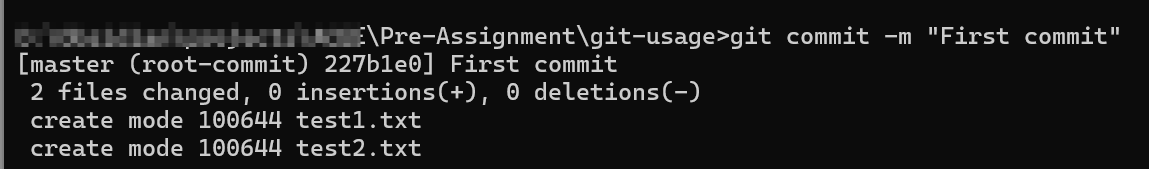
\includegraphics[width = \textwidth]{./figures/commit.png}
\caption{use `git commit' to add commit to the repository}
\end{figure}
\textbf{Question}: What happens if you didn't track the file? Which status of file will be committed?

\textbf{Answer}: If a file is untracked, it will not be included in any commit. Only files in the staged state are committed when you run git commit.

use `git log' to inspect all the commits
\begin{figure}[H]
\centering
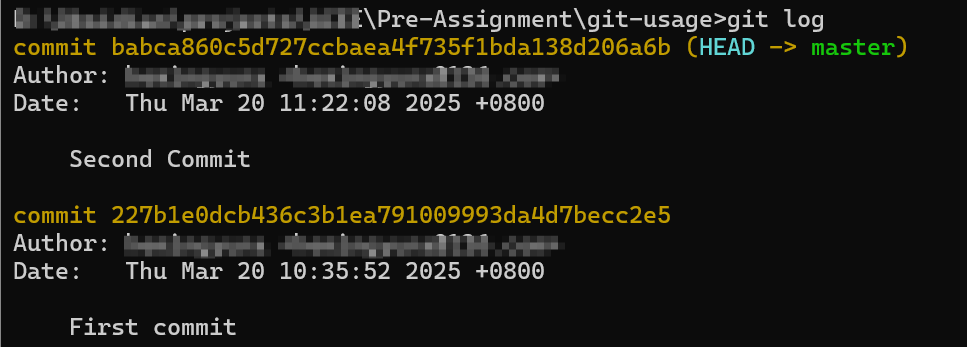
\includegraphics[width = \textwidth]{./figures/log.png}
\caption{use `git log' to inspect the commits}
\end{figure}

\textbf{Question}:  What is the \textbf{HEAD} pointer?

\textbf{Answer}: The \textbf{HEAD} pointer points the current version of the repository. By moving the HEAD pointer to a specific commit, you can review the historical changes of the file.

\subsection{Part 2}
\subsubsection{Task 2}
Make a new branch
\begin{figure}[H]
\centering
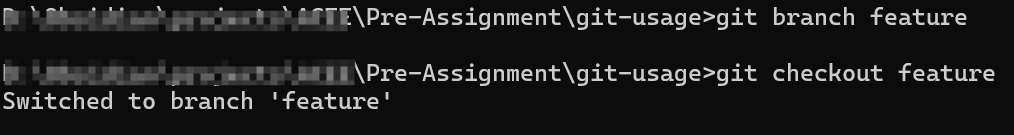
\includegraphics[width = \textwidth]{./figures/new_branch.png}
\caption{use `git branch' to create a new branch}
\end{figure}
\textbf{Question}: What's the difference between committing to main branch and feature branch?

\textbf{Answer}: There's no obvious difference between them. Commits to the feature branch are isolated from the main branch. You can use `git merge' to integrate your changes into main when ready.

When merge the feature branch into main branch, Git reports an error.
\begin{figure}[H]
\centering
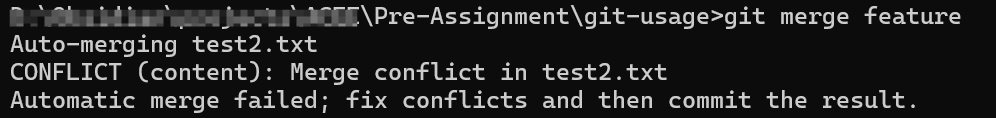
\includegraphics[width = \textwidth]{./figures/conflict.png}
\caption{the conflict when merging two branches}
\end{figure}
Resolve the conflict and complete the merge.
\begin{figure}[H]
\centering
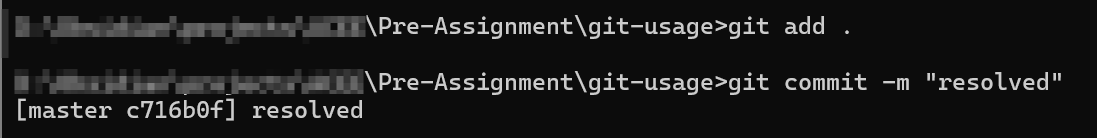
\includegraphics[width = \textwidth]{./figures/resolved.png}
\caption{resolve the conflict}
\end{figure}

\textbf{Question}: What causes conflicts? Why git didn't merge these conflict files automatically?

\textbf{Answer}: Conflicts happen when two branches modify the same part of a file in different ways, and Git cannot determine which version to keep.
You can determine the version that you can keep and resolve the conflict, which makes the merge successful.

Inspect the merge history
\begin{figure}[H]
    \centering
    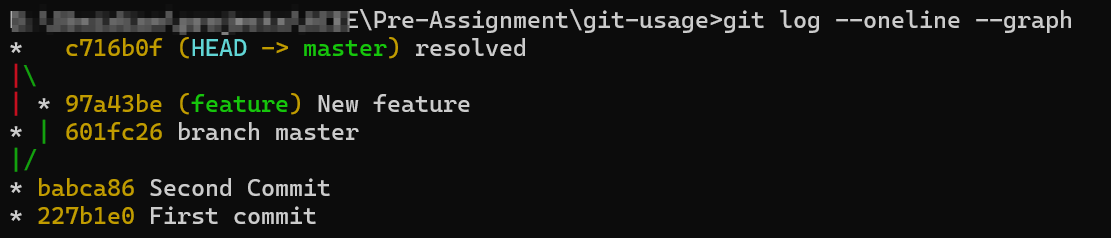
\includegraphics[width = \textwidth]{./figures/graph.png}
    \caption{commit history}
\end{figure}

\subsubsection{Task 3}
Rebase the branch `feature-rebase' onto main. And Git pauses due to the conflict.
\begin{figure}[H]
    \centering
    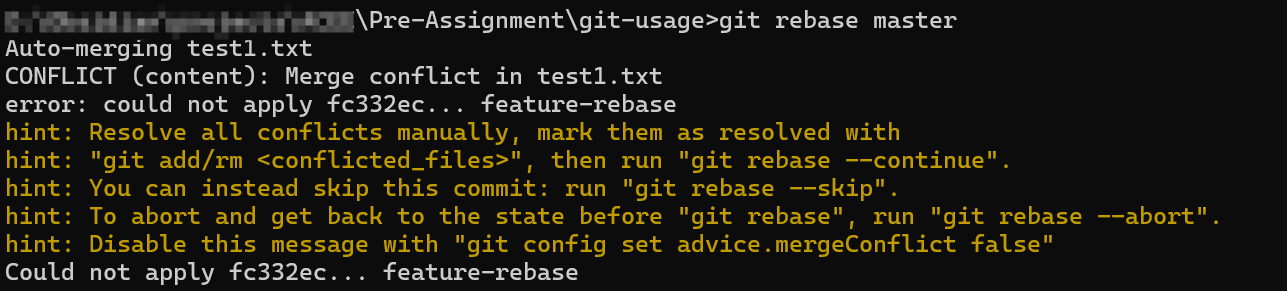
\includegraphics[width = \textwidth]{./figures/rebase-abort.png}
    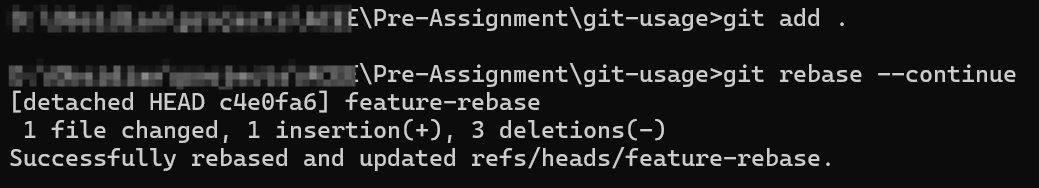
\includegraphics[width = \textwidth]{./figures/rebase-continue.png}
    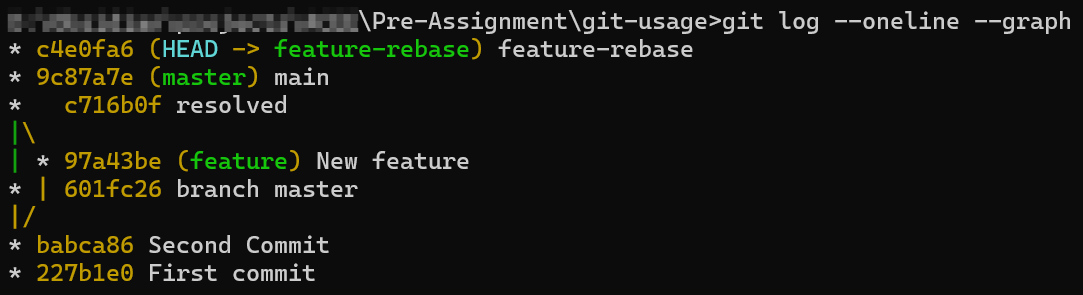
\includegraphics[width = \textwidth]{./figures/rebase-history.png}
    \caption{Rebase}
\end{figure}

\textbf{Question}: How does rebasing work? What’s the difference between merge and rebase?

\textbf{Answer}: Rebase works by replaying the changes made in the feature branch onto the master branch, resulting in a linear and clean commit history. In contrast, merge preserves the original branch structure, which can lead to a more complex commit history. Generally, rebase is used only on private branches,
while merge is used on public branches to clarify the division of work.

Merge the rebased branch
\begin{figure}[H]
    \centering
    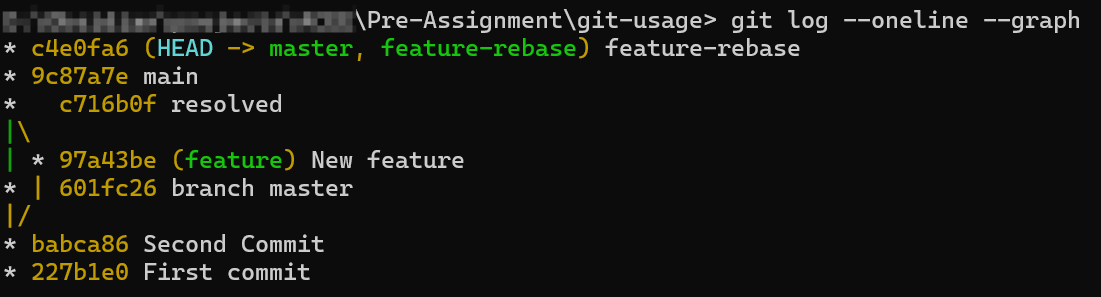
\includegraphics[width = \textwidth]{./figures/fast-forward-merge.png}
    \caption{Merge the rebased branch}
\end{figure}

\textbf{Question}:  In which condition could ``Fast Forward''? What's the advantage of rebasing compared to merge directly
\textbf{Answer}: A fast-forward merge occurs when the target branch is the direct ancestor of the merging branch.
Since all changes are already in a linear history, Git simply moves the branch pointer without creating a merge commit.
Compared to merge directly, rebasing creates a linear history which is cleaner than the one created by merging directly.

\subsection{Part 3}
\subsubsection{Task 4}
Connect the local repository to the remote one, and push.
\begin{figure}[H]
\centering
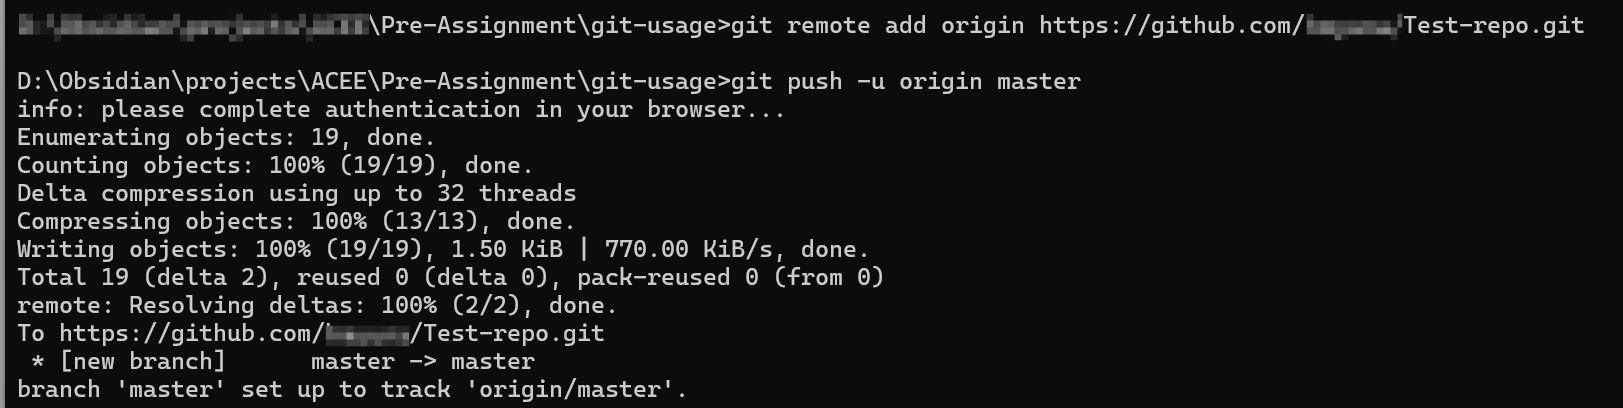
\includegraphics[width = \textwidth]{./figures/remote.png}
\caption{push the repository to the remote branch}
\end{figure}
\textbf{Question}: What does push do? Why might you need the -u flag?

\textbf{Answer}: Push synchronizes the local commits to the remote repository, and the -u flag links the local branch with the remote branch to simplify operations.

Push the local repository to the remote repository.
\begin{figure}[H]
\centering
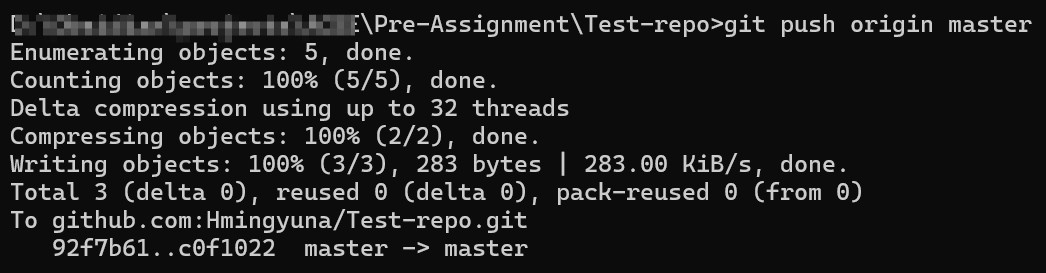
\includegraphics[width = \textwidth]{./figures/push.png}
\caption{push to the forked repo}
\end{figure}
\textbf{Question}: What's the relationship between forked repository and origin repository. Will changes in forked repository affect origin repository

\textbf{Answer}:The forked repository is a branch of the origin. Changes made in the forked repository won't affect the original repository, but you can synchronize the modified parts by submitting a pull request.

Create a pull request.
\begin{figure}[H]
\centering

\includegraphics[width = \textwidth]{./figures/PR2.png}
\caption{PR}
\end{figure}
\textbf{Question}: What's the purpose of a pull request?

\textbf{Answer}:A pull request is used to propose and discuss changes before merging them into the target repository, helping code review and collaboration.

Pull changes from the remote.
\begin{figure}[H]
\centering
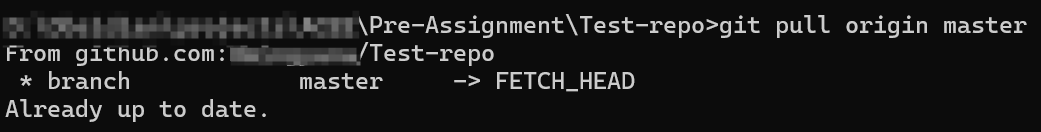
\includegraphics[width = \textwidth]{./figures/pull.png}
\caption{pull the changes}
\end{figure}
\textbf{Question}: What does pull do? Explain how pull request contributes in team cooperation?

\textbf{Answer}: Git pull fetches changes from a remote repository and automatically merges them into the local branch.
A pull request, makes team cooperation easier by allowing team members to review, discuss, and approve proposed changes before they are merged into the main branch,
ensuring the code quality.